\chapter{Approach}
\label{chap:approach}
This chapter outlines our comprehensive software architecture and implementation. Section \ref{sec:software-arch} showcases all the required components for constructing the Scriburg search engine. In Section \ref{sec:crawler-implementation}, we will clarify the functionality of Scriburg's web crawlers. This will contain the workflow, practical challenges encountered during crawling, and corresponding solutions. Moving on to Section \ref{sec:indexer-implementation}, we will demonstrate the indexing workflow. Finally, in Section \ref{sec:ui}, we will delve into the user interface design, highlighting the configurations made available to users and how they enhance the overall user experience.

\section{Software Architecture}\label{sec:software-arch}

Figure \ref{fig:software-arch} shows an overview of the software architecture employed by our search engine. Microservices architecture was used to simplify scalability and split each component's responsibilities. \textbf{Docker} is used to simplify adding and removing crawling nodes. \textbf{Ubuntu 18.04} image is used for each image. Below is a compilation of the utilized technology stack:

\begin{figure}[h]	
     \centering
     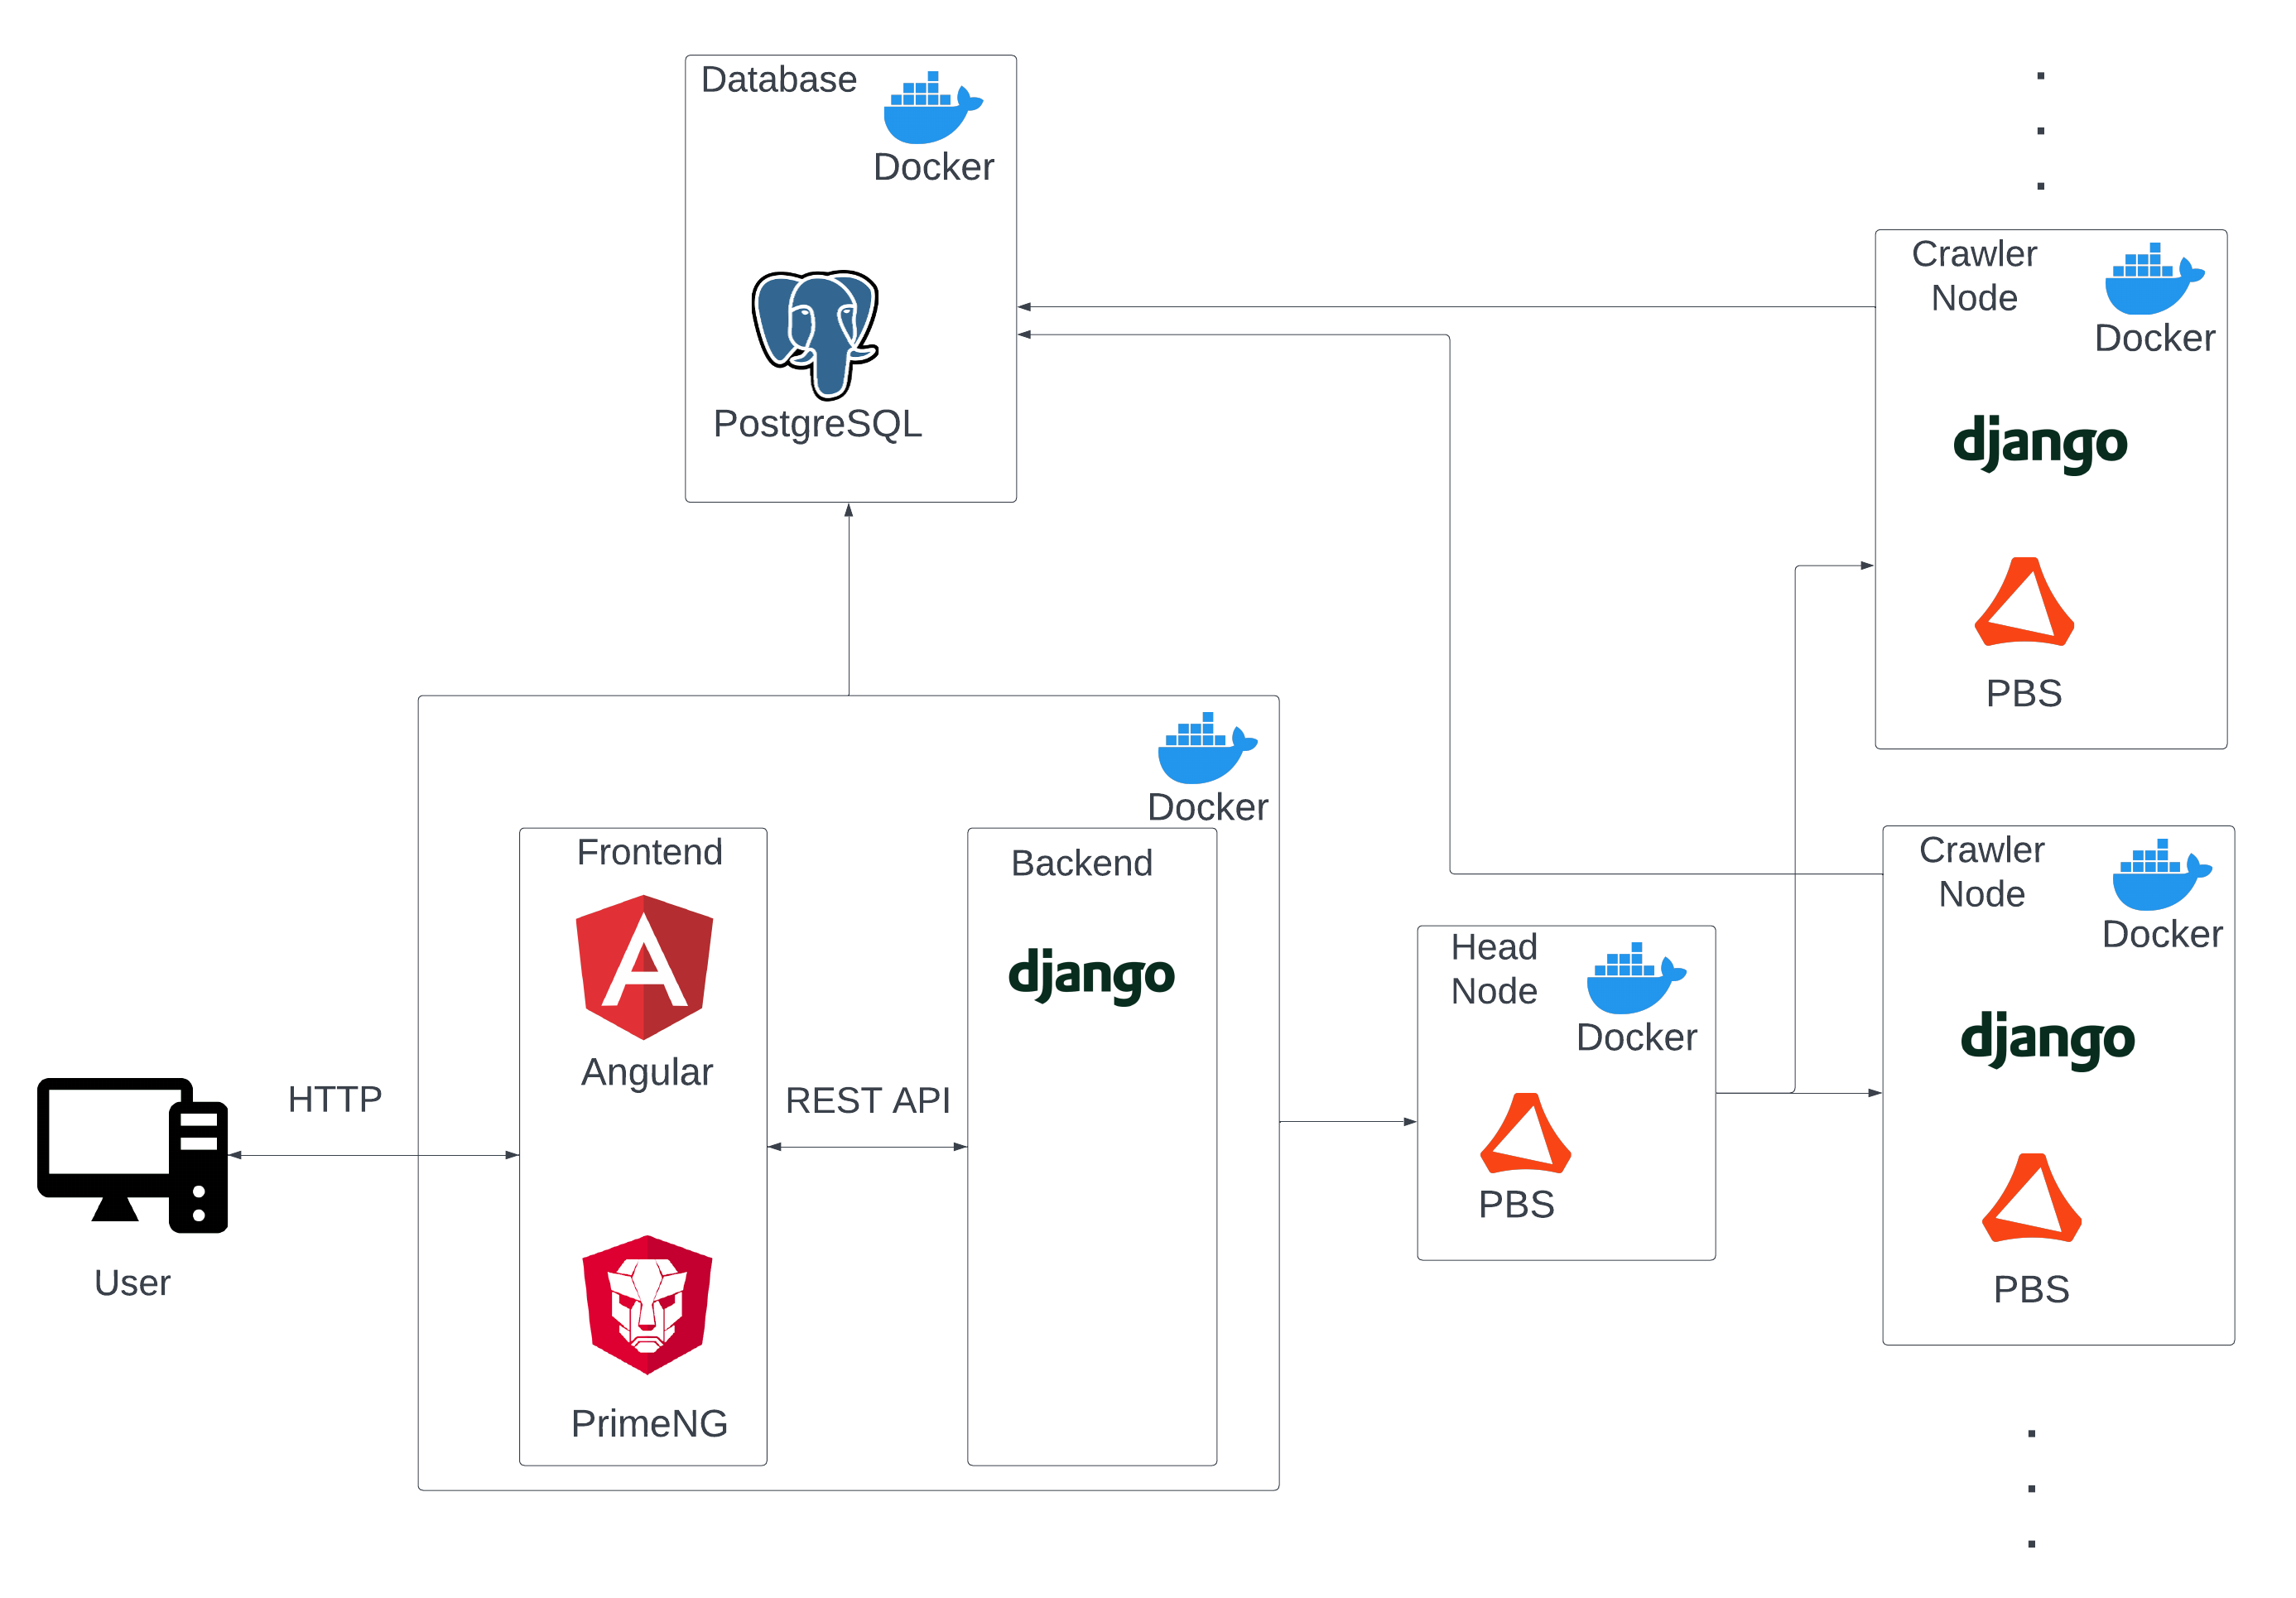
\includegraphics[width=13cm]{figures/software_arch.png}
     \caption{Scriburg software architecture overview.}
     \label{fig:software-arch}
\end{figure}

\begin{itemize}
  \item[] \textbf{Frontend (Angular \& PrimeNG)}: One of the challenges in this thesis involves creating a user-friendly interface for configuring the search engine, targeting non-expert users. We will implement an attractive HTML component with an intuitive interface using the \textbf{PrimeNG} framework to address this challenge. Another design decision is to employ client-side rendering\footnote{Client-side rendering (CSR) is an approach where web content is primarily rendered and processed in the user's web browser, allowing for dynamic, responsive user experiences but potentially longer initial load times. It's commonly used in single-page applications and may pose SEO challenges due to content generated via JavaScript.} with \textbf{Angular} to enhance user experience and responsiveness.
  \item[] \textbf{Backend (Django)}: Serving as the core intelligence of the search engine, the backend houses both the crawler and indexer modules. It facilitates interaction with the \textbf{PBS Head node} to initiate crawling based on user-defined configurations. Moreover, it establishes a connection with \textbf{PostgreSQL} database for storing crawler and indexer configurations, along with job-related information. The selection of the \textbf{Django} as a backend framework was used for several factors. It offers a user-friendly admin dashboard by default, simplifying adding and removing nodes from the cluster. Additionally, Django provides a robust API library, facilitating seamless communication with Angular. The choice of Python as the primary language was influenced by its simplicity, enabling future developers to modify and expand the codebase easily.
  \item[] \textbf{Selenium}: Lives under the backend component, served as a web browser automation tool employed to establish a web session that emulates a genuine user session, allowing for the rendering of specific pages intended for crawling and the downloading of documents to be indexed.
  \item[] \textbf{Head Node (PBS)}: Since crawling is a job that can run in multiple nodes and a distributed system is used, a job scheduler must be used in the design. The \textbf{PBS head node} is the central node that distributes the workload between crawler nodes. \textbf{Portable Batch System (PBS Pro.)} is a job scheduling and workload management system in \textbf{high-performance computing (HPC)} environments. It allows users to submit and manage batch jobs on a cluster of computers, making it easier to utilize the available computing resources efficiently. PBS typically provides job submission, queuing, resource allocation, prioritization, and status monitoring features. It helps administrators and users manage and optimize the execution of computational tasks on a cluster, like crawling in our use case. Other alternatives like \textbf{Slurm} can be used instead of PBS as a job management system.
  \item[] \textbf{Crawler Node (PBS)}: The PBS crawler nodes are responsible for web crawling and storing documents within a PostgreSQL database. They are powered by the Django backend for the crawling process. Manually adding crawler nodes is possible, and after adding a node, one can initiate crawling jobs on it as needed.
\end{itemize}

The application setup initiates with a minimal requirement of four microservices to operate the entire search engine. A Docker container containing both Angular and Django communicating via API. Django communicates with the database to store the crawling and indexing configurations and saves the submitted job metadata and statistics. The PBS head node must be configured at least to use one crawler node. The crawler node will perform the crawling job and save the results to the shared database. The more computing power needed, the more nodes can be added to scale the system horizontally\footnote{Horizontal scaling involves expanding a system's capacity by introducing more machines (nodes) instead of enhancing the capabilities of the existing machines.}. 

The workflow begins with a user-friendly interface presented by Angular and PrimeNG, encompassing all the configurations and tools enabling users to crawl quickly and index various websites. Users can modify configurations and submit a crawling job to the head node. The head node, in response, identifies an available Crawler Node to execute the task. It is worth noting that the PBS cluster can be bypassed, and the crawling process can be run locally on a localhost server. Users can monitor the progress of the running job from the browser. Once crawling is completed and the user is happy with the result, the user can start indexing. The indexing job does not support a distributed architecture and will be executed locally and not on the PBS cluster.

The primary reason for bypassing the distribution of the indexing task is that, in contrast to the intensive computing requirements of crawling, indexing the gathered data often demands significantly less computational power. It is important to note that this is not an absolute rule, as it relies on the volume of documents to be indexed. However, in the case of specialized crawlers like Scriburg, designed for specific domains rather than comprehensive web crawling, this step can often be avoided.

\pagebreak
\section{Crawler Implementation}\label{sec:crawler-implementation}

As illustrated by the pseudo-code shown in Algorithm \ref{alg:crawler}, the crawler starts by loading the configuration submitted by the user from the database. More details about the configuration are in the user interface Section \ref{sec:ui}. Based on the crawler configuration, a thread pool will be created. The thread pool contains all the threads crawling the site, where each thread contains a queue of URLs that it crawls from. The thread pool ensures that if one thread has no URLs, it can ask other threads to split the workload. The choice between a Breadth First Search (BFS) or Depth First Search (DFS) algorithm in the crawler depends on the user's configurations. However, for clarity, Algorithm \ref{alg:crawler} assumes using a BFS approach, and accordingly, a queue is used instead of a stack.


\begin{algorithm}[H]
	\caption{Start Crawling}\label{alg:crawler}
	\begin{algorithmic}[1]
		\State load\_crawler\_configurations() \Comment{Configurations submitted by the user}
		\State $thread$ $\gets$ create\_threads\_pool() \Comment{Generate a thread and add it to the threads pool}
	    \State $urls\_queue$ $\gets$ get\_thread\_urls\_queue($thread)$)
	    \State $seed\_url$ $\gets$ get\_seed\_url()
	    \State add\_url\_to\_queue($urls\_queue$, $seed\_url$)
	    \State $robots\_file$ $\gets$ load\_robots\_file\_content()
	    \While {$urls\_queue$ not empty or all threads not done}
		\If{$urls\_queue$ is empty}
		    \State $urls\_queue$ $\gets$ get\_thread\_urls\_queue($thread$)
		\Else
			\State $current\_url$ $\gets$ $urls\_queue$.next()
			\State load($current\_url$) \Comment{Load and render the page}
            \State execute\_automated\_actions() \Comment{If enabled, clicking, waiting, and scrolling actions are executed}
			\State $new\_links$ $\gets$  find\_all\_page\_links() \Comment{Collect all links in the current page}
   			\State filter\_unwanted\_urls($new\_links$) \Comment{Remove duplicated, disallowed and cross-origin links}
			\State $docs$ $\gets$ find\_page\_documents() \Comment{Download all documents in the page}
			\State filter\_unwanted\_documents($docs$)
		\EndIf
		\EndWhile
	\end{algorithmic}
\end{algorithm}


A seed URL is pushed into the present thread queue, representing the initial point for the crawling procedure as specified by the user configuration. This seed URL enables retrieving the \texttt{robots.txt} content, which is downloaded once and utilized throughout the crawling operation. Typically, \texttt{robots.txt} files are located at the root path of the URL, but it is also possible to configure the crawler to fetch them from a user-defined location. Without a specific user configuration, the default behavior involves automatically reading the \texttt{robots.txt} file from the root.

Each crawler goes into an infinite loop that will continue to run either if the queue still contains URLs to be fetched or if at least one crawler is still running. This guarantees that although one thread is busy, it contains many URLs that need help with crawling, and the free threads can share the load with it. If the thread queue becomes empty, the thread will ask the pool to find the following URLs to fetch. Otherwise, the next URL in the queue will be fetched, and a Selenium page request will be made. Afterward, automated actions such as scrolling down, waiting, and clicking defined by the user are executed. Those actions give the user the power to control the browser to mimic real agent behavior. The action chain will be discussed more in the user interface design Section \ref{sec:ui}.    

Once the page has fully loaded and the specified actions have been executed, the crawler proceeds to retrieve all the next links, filter them, and then push them into the queue. The final step involves downloading the documents intended for indexing.

\subsection{Threads Pool}\label{sec:threads-pool}
The threads pool for sharing URLs includes all the crawlers running on a single machine, not all the clusters. Currently, each node operates independently, so if two crawlers run on different nodes, the visited URLs can be revisited by other nodes. To address this issue, a solution is to transfer the in-memory visited URLs dictionary to a key-value database, such as \textbf{Redis}. Instead of including visited URLs in a dictionary shared by the thread pool, they can be stored in the Redis database, which is accessible to all other crawling nodes.

When a thread queue becomes empty, instead of idling, the thread will pause for five seconds and then inspect the threads in the thread pool. The thread with the largest queue will divide it into two halves with the available free thread. If a thread is available and another thread has fewer than five URLs, no division will occur, as the threshold is set at five. Adjusting the splitting threshold to higher values like 20 or 50 would diminish the benefits of multithreading and not enhance performance, as this will result in more ideal free threads. Reducing the threshold to smaller values like 1 or 2 would lead to frequent queue sharing among all threads, increasing the unnecessary overhead of link sharing. After experimenting with four threads, the optimal balance was a split threshold between five and ten.

\subsection{Scaling the System}
One of our primary goals was to create a system capable of performance scalability by adding low-cost workstations to support extra components. Whether to scale vertically by adding more threads or horizontally by introducing more machines, it can be challenging to decide which scale to use and when. We projected that a single instance of Scriburg would suffice for approximately four to eight crawlers. However, a second crawl manager (a separate crawling system node) would be needed beyond this point. Other approaches, such as those mentioned in \cite{shkapenyuk2002design}, recommend introducing additional crawler managers or new crawler nodes when the number of crawlers reaches eight.


\subsection{Practical Challenges}
\begin{itemize}
  \item[] \textbf{Canonical URLs}: As previously mentioned, avoiding revisiting already-seen pages prevents content duplication and eliminates the risk of the crawler getting stuck in a loop, thereby enhancing the efficiency of the crawling process. Nevertheless, the task of identifying previously visited URLs is complicated by dynamic URLs, where different URLs can ultimately lead to the same page. To address this challenge, every fetched URL must undergo normalization and be transformed into its fundamental form. In \ref{lst:con-url}, we illustrate various examples of different URL forms that ultimately point to the same URL. In Scriburg, we adopt a straightforward approach by disregarding parameters and fragments from each fetched URL.

\lstset{language=HTML}
\begin{lstlisting}[frame=single, caption={Example of different forms of the same URL.},captionpos=b, label={lst:con-url}]
https://uni-freiburg.de
https://uni-freiburg.de/
https://uni-freiburg.de/#fragment
https://uni-freiburg.de/index.html
https://uni-freiburg.de/index.html?tab=research
https://uni-freiburg.de/index.html?tab=research&user=12
\end{lstlisting}

\item[]  \textbf{Duplicated Content}: Around \textbf{29.2\%} of the web content is duplicated and it is growing \cite{fetterly2003evolution}. While a web crawler avoids revisiting identical URLs to prevent content duplication, it is important to note that identical content may exist in different URL paths within the same website. For instance, a men's shoe might be accessible via various links like "\texttt{/winter/shoes/}", "\texttt{/men/shoes/}", or "\texttt{/sales/shoes/}". Relying solely on the URL as a unique identifier to prevent content duplication is unreliable. Moreover, as we discussed, URLs can have different forms, and sometimes, we revisit the same page unintentionally.
A more effective approach involves comparing the content with the database after parsing. Instead of a straightforward content check against the database, which can pose performance challenges, we employ a more efficient method. We generate a unique hash code using the \textbf{SHA-1}\footnote{
SHA-1 (Secure Hash Algorithm 1) is a cryptographic hash function that takes an input and produces a fixed-length 160-bit (20-byte) hash value, typically represented as a 40-character hexadecimal number. It was widely used for data integrity and security purposes.} hashing algorithm based on the content string intended for storage. This hash code is then stored in the database.
Before saving a new document, we can verify if the hash code exists in the database. This method ensures content uniqueness, even when it appears under different URLs on the same site, without the computational overhead of directly comparing lengthy content strings in the database. Note that sometimes, when the page admin edits their content, even one character edited will be classified as a new document.

\item[]  \textbf{Dynamic Content}: Crawling dynamic websites presents a distinct set of challenges compared to static websites. Dynamic sites generate content on the client side through technologies like JavaScript, adding complexity to the task of accessing and extracting data. A primary concern lies in uncovering concealed content that necessitates user interaction. For instance, certain websites hide lengthy content portions, revealing them only upon clicking a \textit{"read more"} button. Additionally, most websites implement lazy loading, fetching content on-demand via \textbf{AJAX}\footnote{AJAX (Asynchronous JavaScript and XML) requests are a technology for sending and receiving data from a web server without requiring a full page refresh, enabling dynamic and asynchronous data updates in web applications.} requests.
Selenium establishes a genuine session to address these challenges and fully renders the web page. This approach emulates user interactions using action chains, which simulate waiting, scrolling, and clicking. More details will be discussed in the User Interface Design Section \ref{sec:ui}.

\item[]  \textbf{Robustness}: The dynamic nature of web content can present numerous exceptional scenarios for crawlers, making ensuring comprehensive coverage of these edge cases challenging. Nonetheless, we simplified troubleshooting by implementing logs and employing effective monitoring and termination criteria. We minimized the risk of falling into unnecessary web traps, a particularly crucial aspect when integrating cloud-based computing solutions like \textbf{Amazon Web Services AWS}. Crawlers can be halted by establishing specific criteria to ensure termination. The initial criterion involves defining a maximum depth, which restricts the number of page transitions to a single level. Additionally, monitoring and restricting the total count of visited pages and collected documents is possible. Another method is to use a wall-time measurement to monitor the crawler's runtime duration and trigger an abort if the crawler exceeds the expected time frame. 

\item[]  \textbf{Avoiding DoS}: Increasing the number of requests and expanding the crawler's capacity by adding more threads or nodes may boost performance. However, this approach carries a significant risk of overwhelming the targeted servers, potentially resulting in \textbf{Distributed Denial of Service (DDoS)} or \textbf{Denial of Service (DoS)} attacks. Servers can perceive this surge in requests as an attack, which could lead to the crawler being blocked and subsequently banned.
To mitigate this risk, it is crucial to introduce a waiting period between each request made by the same crawler. Additionally, when using Selenium, a deliberate delay of at least one second or more is already integrated to allow for the complete rendering of web pages. Nevertheless, more than these precautions are required to prevent users from adding more nodes and executing DDoS attacks on the servers. Consequently, it is strongly advisable to exercise cautious management by monitoring and regulating the number of threads and nodes. This approach demonstrates respect for the targeted servers and helps prevent overloading them.

\end{itemize}

\section{Indexer Implementation}\label{sec:indexer-implementation}

Unlike crawling, which can be computationally intensive, indexing thousands of documents is relatively lightweight. Hence, it is carried out on the localhost without any multithreading support.
Algorithm \ref{alg:indexing} clarifies the process of creating an inverted list. Firstly, the indexer loads the user-defined indexing configurations from the database. We will list more configurations in Section \ref{sec:ui}. Subsequently, an empty inverted list is initialized. Within Python, one can implement it as a dictionary, with each word as a key and an associated value representing a list of document IDs that include that word (postings). While one can include additional metadata in the list, such as word frequency and positions of the words in the document, we will omit these details for algorithmic simplicity.


\begin{algorithm}[H]
	\caption{Create Inverted List}\label{alg:indexing}
	\begin{algorithmic}[1]
	    \Require $documents$ not empty
		\State $config$ $\gets$ load\_indexer\_configurations() \Comment{Load user chosen configurations}
		\State $inverted\_list$ $\gets$ \{\} \Comment{We initialize an empty dictionary}
		\State $threshold$ $\gets$ get\_small\_words\_threshold($config$)
	    \State $stop\_list$ $\gets$ stop\_words\_list($config$)
     	\State $docs\_length$ $\gets$ [ ] \Comment{We initialize an array of documents lengths}

        \For{$doc$ in $documents$}
          \State $doc\_length$ $\gets$ 0
          \State $tokens$ $\gets$ tokenize($doc$) \Comment{Split the document into tokens}
          \For{$token$ in $tokens$}
          	\If{$token$ > threshold and $token$ not in $stop\_list$}
		    	\State add\_token\_and\_doc\_id\_to\_inverted\_list($token$, $doc.id$)
		    	\State $doc\_length$ $\gets$ $doc\_length$ + 1
			\EndIf
          \EndFor
          \State $docs\_length$.add($doc\_length$)
        \EndFor
        \State calculate\_bm25\_score($inverted\_list$) \Comment{Compute the BM25 score}
        \State cache($inverted\_list$) \Comment{Cache the indexer for future usage}

	\end{algorithmic}
\end{algorithm}

The user specifies three variables: \textit{threshold} and \textit{stop\_list}, which are retrieved from the database. The \textit{threshold} represents the minimum word length required for tokenization from a document. The \textit{stop\_list} is a predefined list of terms that should be omitted from the indexing process.
Afterward, we iterate through all the documents, performing the following steps for each one:
Initializes the document length as a counter, initially set to zero.
Tokenizes the document to obtain a list of words.
Iterates through the word list, checking each word's length against the \textit{threshold} and verifying if it is not in the \textit{stop\_list}. If these conditions are met, the word is added to the inverted list, and the document length counter is incremented by one.

Once the inverted list is constructed, we calculate the \textbf{MB25} score for each token in a document based on equation \ref{eq:bm25}. Afterward, it is saved into a cache for future retrieval and use.

\section{User Interface Design}\label{sec:ui}
This thesis extends beyond merely building and designing a search engine. It also encompasses the critical goal of enabling users to configure and utilize it effortlessly. This section will explore the user interface design, workflow, and user-facing configurations.

\subsection{Templates and Inspectors}
The user begins their workflow on the homepage, where they can access documentation explaining how to use the application. The application's first component to be created is the \textbf{Template}, which serves as a blueprint for specifying the document fields to be extracted from web pages. Establishing a unique template for each page is a prerequisite, although the same Template can also be applied across different websites. These templates consist of a list of \textbf{Inspectors}. An inspector can be thought of as a field. For example, creating a template for parsing a title and a product price will require two different inspectors. Each inspector contains the attributes shown in Table \ref{table:inspector-fields}.


\begin{table}[ht]
\centering
{\footnotesize
\begin{tabular}{|P{2.5cm}|P{9.9cm}|}
    \hline
     \textbf{Name\textsuperscript{*}} & Represents the inspector's identifier, such as \textit{"Title"} or \textit{"Price."}  \\ \hline

     \textbf{Selector\textsuperscript{*}} & It contains the XPath\footnote{XPath is a language used for navigating and selecting elements from an XML document, often employed for web scraping and data extraction from HTML documents.} expression identifying the chosen element value.\\ \hline

     \textbf{Type\textsuperscript{*}} & This can take values like \textit{"Text,"} \textit{"Link,"} or \textit{"Image,"} signifying the nature of the content to be extracted.\\ \hline\hline

     \textbf{Variable Name} & An optional shorthand representation of the selector, facilitating its use during the indexing process to enhance search results (Ranking). \\ \hline

     \textbf{Clean-up Expression List} & Used to refine the extracted value from the inspector. This proves beneficial in eliminating unwanted noise (remove the currency when extracting a price).\\ \hline

     \textbf{Attribute} & Allows the user to specify an HTML element attribute, such as \textit{"src,"} \textit{"name,"} or \textit{"href,"} as an optional parameter to be saved into the database.\\ \hline
\end{tabular}}
  \captionsetup{justification=centering,margin=2cm}
  \caption{Inspector form fields. Fields with * are required.}
  \label{table:inspector-fields}
\end{table}


The \textbf{Actions Chain} list can be used depending on the targeted website's characteristics. An \textbf{Actions Chain} constitutes an array of sequenced actions replicating user interactions. This functionality is valuable for tasks such as accepting cookies, scrolling to load additional content or waiting for the website to render in cases where the process may exceed the expected duration. 

\subsection{Crawlers}
Once the Template is created, the subsequent step is to access the Crawlers page and create a new Crawler. A \textbf{Crawler} comprises various essential configurations as shown in Table \ref{table:crawler-configurations}.

\begin{table}[ht] 
\centering
{\footnotesize
\begin{tabular}{|P{2.5cm}|P{9.9cm}|}
    \hline
     \textbf{Name\textsuperscript{*}} & A user-defined identifier for the crawler  \\ \hline
     \textbf{Template\textsuperscript{*}} & The blueprint for collecting documents with \\ \hline
     \textbf{Seed URL\textsuperscript{*}} & The starting point of crawling  \\ \hline\hline
     \textbf{Max Pages} & The upper limit for the number of pages to be visited  \\ \hline
     \textbf{Max Docs} & The maximum number of documents to be collected \\ \hline
     \textbf{Max Depth} & Maximum jumps between pages (crawling depth) \\ \hline
     \textbf{Robots.txt} & The URL where the \texttt{robots.txt} file can be located  \\ \hline
     \textbf{Threads} & Number of threads used in the crawling process \\ \hline
     \textbf{Pagination} & Scope to collect the following URLs  \\ \hline
     \textbf{Excluded URLs} & URLs that the crawler must refrain from visiting \\ \hline
     \textbf{Walltime (ms)} & Sets the duration for which the crawler should continue crawling\\ \hline
     \textbf{Show Browser} & Deactivate the headless mode in Selenium \\ \hline  
\end{tabular}}
  \captionsetup{justification=centering,margin=2cm}
  \caption{Crawler configurations options. Fields with * are required.}
  \label{table:crawler-configurations}
\end{table}

\subsection{Runners}
Once the crawler is set up with the appropriate configurations tailored to the targeted website, the next step is to create a job referred to as a \textbf{Runner}. Multiple runners can be associated with each crawler, allowing them to run on different nodes. It is important to note that each runner can use multithreading based on the crawler's configurations and employ distinct crawler settings. This approach provides an effective means to assess the crawler's performance until the desired outcome is achieved. Every runner instance necessitates the presence of the crawler and a designated machine IP where it will execute. The chosen machine must be registered within the \textbf{PBS Head Node} and online. By default, \textbf{localhost} is set as the value, where some will use their local machine as a crawling node.

\begin{figure}[ht]	
     \centering
     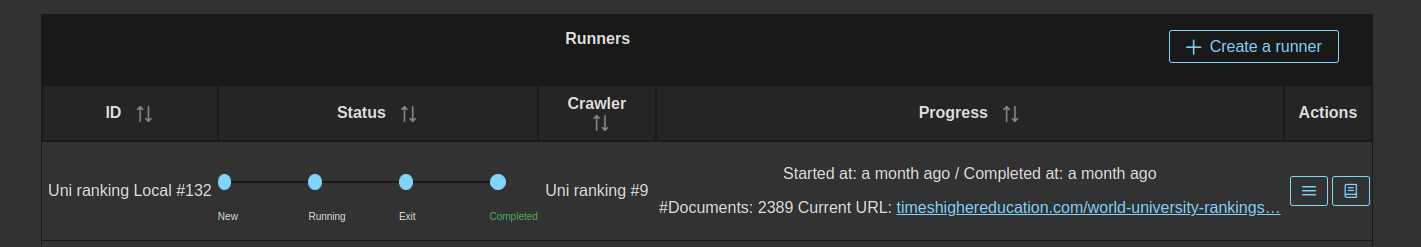
\includegraphics[width=13cm]{figures/demo-8.png}
     \caption{An overview of the runners table, showing the runner's status and progress.}
     \label{fig:runners-overview}
\end{figure}


It is essential to keep a close eye on the crawler runner to monitor its performance and configuration effectiveness before finalizing it. This proactive approach helps save time and guarantees that the crawler collects targeted data accurately. The \textit{\textbf{Runners}} table provides a straightforward and informative progress overview through four primary status indicators. The initial status is \textit{\textbf{New}}, representing the runner's initialization before the crawling process begins. \textit{\textbf{Running}} signifies that the crawling process is currently undergoing. \textit{\textbf{Exit}} indicates a status change that occurs when an error occurs, leading to the termination of the crawling process. Finally, \textit{\textbf{Completed}} marks the last status, indicating that the runner has finished its task and exited. During the crawling process, various statistics about the runner are collected, including information such as the total number of visited pages, the average number of documents discovered per page, and the various HTTP status codes encountered. One can retrieve the documents collected by the runner by selecting the \textbf{Download CSV} option from the actions drop-down menu.


\subsection{Indexers}
Once the runner has finished its job and the user is satisfied with the results, the collected documents can be indexed and prepared for future searches. To access this feature, one can navigate to the \textbf{Indexers} view, where the indexers table displays the current indexers and their respective statuses.


\begin{figure}[h]	
     \centering
     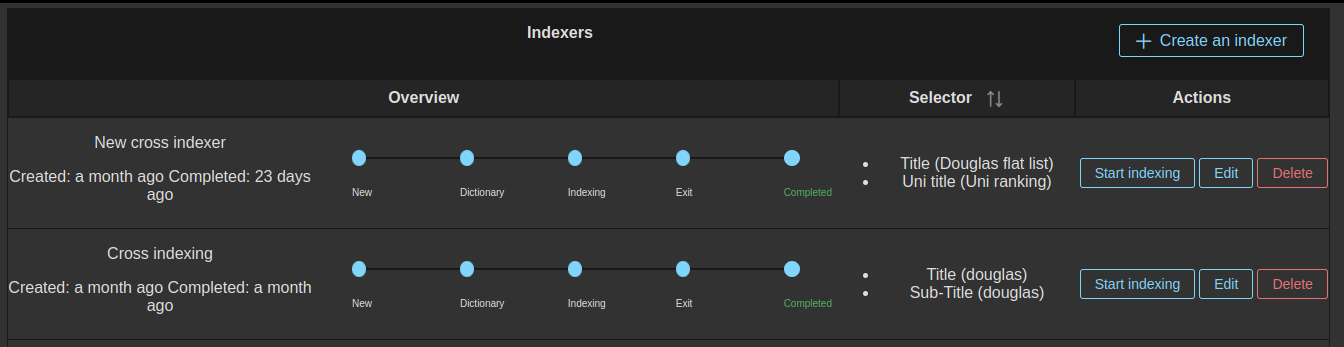
\includegraphics[width=13cm]{figures/demo-10.png}
     \caption{An overview of the indexers table, showing their status and progress.}
     \label{fig:indexers-overview}
\end{figure}

In this context, inspectors come into play. These inspectors are responsible for mapping the fields extracted from the document, such as \textit{Title}, \textit{Price}, and \textit{Image}. Users can select which inspectors to index from a drop-down menu, with the choice limited to only text fields. Images and links are excluded from this indexing. Note that if one template is used to fetch from different websites when indexing the collected documents, one can select the inspectors related to this template, and the indexing process will contain all the websites that use this template, which is a nice feature.

\begin{table}[ht] 
\centering
{\footnotesize
\begin{tabular}{|P{2.5cm}|P{10.8cm}|}
 \hline 
\textbf{Name\textsuperscript{*}} & A user-defined identifier for the indexer\\ \hline
\textbf{Inspectors\textsuperscript{*}} & Checklist of all the available inspectors used by the crawlers. \T\B 
\\ 
\hline
\hline
\textbf{b Parameter} & b parameter for the BM25 formula. \T\B 
\\ 
\hline
\textbf{k Parameter} & k parameter for the BM25 formula. \T\B 
\\ 
\hline
\textbf{Stop Words List} & List of words that should be excluded during the indexing process. \T\B 
\\ 
\hline
\textbf{Small Words Threshold} & The threshold of which the word can be considered small and will be skipped from the indexing process. \T\B 
\\ 
\hline
\textbf{Words Weight List} & Boost some words by giving them weight, e.g. \textit{"Freiburg=5"} will add more 5 points to the score when the \textit{"Freiburg"} word is found. \T\B 
\\ 
\hline
\textbf{Boosting Formula} & This formula result will be added to the final score. It uses inspectors variable. \T\B 
\\ 
\hline
\textbf{Dictionary File Name} & The dictionary file name that helps the suggestions list by using synonyms.\\ \hline
\textbf{Use Synonyms} & Enable using synonyms in the suggestions list. For example, typing \textit{"USA"} will result in \textit{"United States of America"}.\\ \hline
\textbf{Q-Gram} & The \textit{n} value of the q-grams for creating a q-gram inverted index, see Section \ref{sec:q-gram-fuzzy}\\ \hline
    \end{tabular}
}
  \captionsetup{justification=centering,margin=2cm}
  \caption{Indexer configurations options. Fields with * are required.}
  \label{table:indexing-config}
\end{table}

While some of the indexing configurations in Table \ref{table:indexing-config} are already explained within the table, others may benefit from further clarification. The \textbf{Words Weight List} refers to a list of words along with their associated weights. If a term containing one of these words is present in a query, its score will be added and contribute to the overall query score. Adding more weights to some words can be beneficial as users find them more important than others. 

The \textbf{Boosting Formula} feature can be used with inspector variables to influence the ranking process. For example, suppose one wants to rank products based on text relevance and factors like reviews or prices (which are numeric values rather than text). In that case, one can utilize the Boosting Formula. To do this, one can assign a variable name to an inspector, such as \textit{review}. Then, in the Boosting Formula field, one can insert a formula like $log(review)$, which will convert the numeric value in the inspector field \textit{review} into a numerical score. This score is then incorporated into the ranking formula, contributing to the final ranking score.

\subsection{Search Engine Result Page (SERP)}
All the indexed documents can be easily searched on the search page, consisting of three primary components. First, there is the search bar, which leverages the suggestions list dictionary configured during the indexing phase. The second component is a drop-down menu containing all the cached indexers that have previously been indexed. The last component is the result table, which uses a dynamic layout depending on the inspectors used for each document. For example, if the indexer indexes only the \textit{title} inspector of a product, then the table will only contain one column with the inspector's name as a header. 
\begin{figure}[ht]	
     \centering
     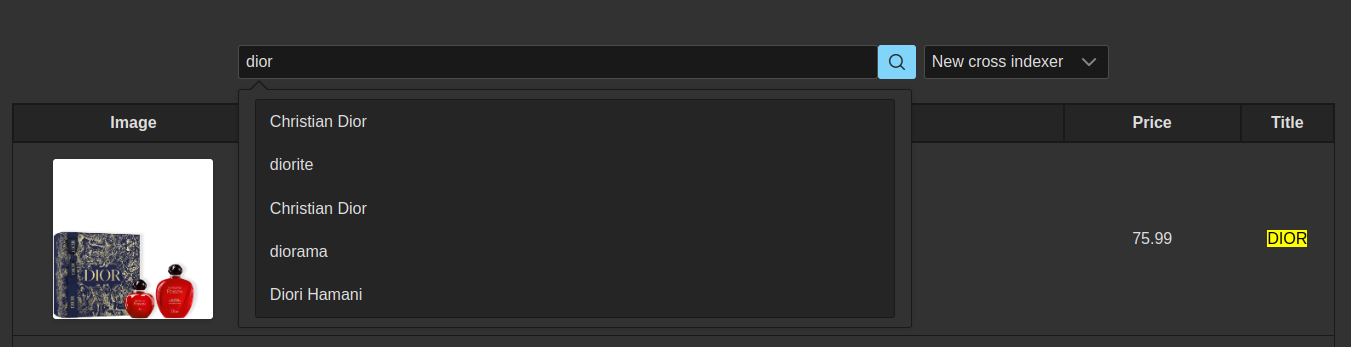
\includegraphics[width=13cm]{figures/demo-12.png}
     \caption{Scriburg Search Engine Result Page (SERP).}
     \label{fig:search-result-view}
\end{figure}


Table \ref{fig:search-result-view} shows the search result of products where we can note that it supports different data types like images. Note that the search result shows the 25 top matching results. 